\documentclass[a4paper, 14pt]{extarticle}
\usepackage{amsmath, amssymb, mathpazo, tikz}

\title{Angles}

\newcommand{\bC}{\mathbb{C}}

\begin{document}
\maketitle


\begin{center}
  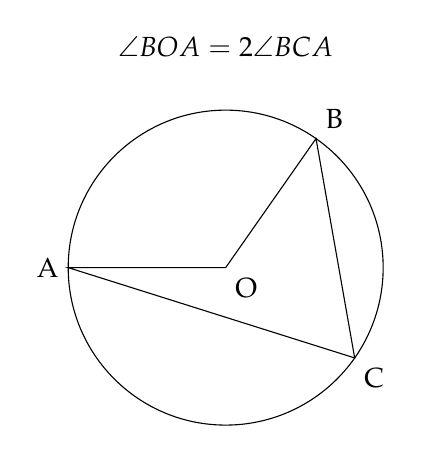
\begin{tikzpicture}
    \node at (0,2.8) {$\angle BOA = 2\angle BCA$};
    \draw (0,0) circle[radius=2];
    \coordinate[label=below right:{O}] (O) at (0,0) {};
    \coordinate[label=left:{A}] (A) at (180:2) {};
    \coordinate[label=above right:{B}] (B) at (55:2) {};
    \coordinate[label=below right:{C}] (C) at (-35:2) {};
    \draw (A) -- (O) -- (B) -- (C) -- cycle;
  \end{tikzpicture}
  \hskip 3em
  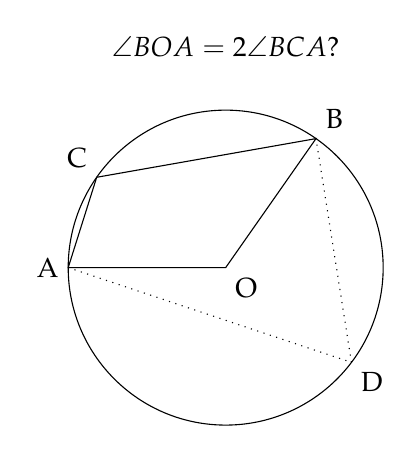
\begin{tikzpicture}
    \node at (0,2.8) {$\angle BOA = 2\angle BCA$?};
    \draw (0,0) circle[radius=2];
    \coordinate[label=below right:{O}] (O) at (0,0) {};
    \coordinate[label=left:{A}] (A) at (180:2) {};
    \coordinate[label=above right:{B}] (B) at (55:2) {};
    \coordinate[label=above left:{C}] (C) at (-215:2) {};
    \coordinate[label=below right:{D}] (D) at (-37:2) {};
    \draw (A) -- (O) -- (B) -- (C) -- cycle;
    \draw[dotted] (A) -- (D) -- (B);
  \end{tikzpicture}
\end{center}

Directed angles are a good thing (and they the thing that the algebra
will be doing for us!)

If we use tangent of the angle, we will be doing directed angles
modulo $\pi$; if we use the tangent of half the angle, we might be
able to do directed angles modulo $2\pi$.

\end{document}
